% tADRguide.tex
% v1.0 released January 2013

\documentclass{tADR2e}

% The following packages can be found on http:\\www.ctan.org
\usepackage{caption}
\usepackage{wrapfig}
\usepackage{color}
\usepackage{graphicx} % for pdf, bitmapped graphics files
%\usepackage{epsfig} % for postscript graphics files
\usepackage{mathptmx} % assumes new font selection scheme installed
%\usepackage{times} % assumes new font selection scheme installed
\usepackage{amsmath} % assumes amsmath package installed
\usepackage{amssymb}  % assumes amsmath package installed
\usepackage{mathrsfs}
\DeclareMathOperator*{\argmin}{argmin}
\usepackage{algorithm}
\usepackage{algpseudocode}  %\usepackage[noend]{algpseudocode}
\algtext*{EndWhile}% Remove "end while" text
\algtext*{EndIf}% Remove "end if" text
\usepackage{booktabs}
\usepackage{multirow}
\usepackage{proof}
\newtheorem{property}{Property}
\usepackage[numbers]{natbib}
\algnewcommand\algorithmicinput{\textbf{input:}}
\algnewcommand\INPUT{\item[\algorithmicinput]}
\algnewcommand\algorithmicoutput{\textbf{output:}}
\algnewcommand\OUTPUT{\item[\algorithmicoutput]}
\makeatletter
%\let\NAT@parse\undefined % allow hyperref to work with ieeeconf.cls for bib numbers
\makeatother
\usepackage{hyperref}
%\usepackage{cite}


% Math shortcuts :
\newcommand\real{\mathbb{R}}
\newcommand\p{\mathbf{p}}
\newcommand\pii{\mathbf{p_{i,i+1}}}
\newcommand\pij{\mathbf{p_{i,j}}}
\newcommand\gT{\tilde{g}^T}
\newcommand\g{\tilde{g}}
\newcommand\CS{\mathcal{C}}
\newcommand\dimCS{n_\mathbf{C}}
\newcommand\body{{\cal B}}
\newcommand\Sone{\mathbf{S}^1}
\newcommand\Sthree{\mathbf{S}^3}
\newcommand\conf{\mathbf{q}}
\newcommand\xx{\mathbf{x}} % \x already defined in the class
\newcommand\cost{C}
\newcommand\weight{W}
\newcommand\translation{\mathbf{t}}
\newcommand\tcolli{t_{coll\ i}}
\newcommand\po{\mathbf{po}}
\newcommand\Jf{{J_f}}
\newcommand\kernel{\mbox{Ker }}

%%%%%%%%%%%%%%%%%%%%%%%%%%%%%%%%%%%%%%%%%%%%%%%%%%%%%%%%%%%%%%%%%%%%%%%%%%%%%%%%
\begin{document}
\graphicspath{{images/}}

\jvol{00} \jnum{00} \jyear{2015} \jmonth{October}

\title{{\itshape Advanced Robotics} A simple path optimization method for motion planning }	

\author{Myl\`{e}ne Campana$^{a,b}$ $^{\ast}$ \thanks{$^\ast$Corresponding author. Email: mcampana@laas.fr}, Florent Lamiraux$^{a,b}$ and Jean-Paul Laumond$^{a,b}$
\\\vspace{6pt}
$^{a}${\em{LAAS-CNRS, Toulouse, France}};
$^{b}${\em{ This work has been supported by the project ERC Advanced Grant 340050 Actanthrope and by the FP~7 project Factory in a Day under grant agreement n°~609206 }}
}
\maketitle

\begin{abstract}
Most algorithms in probabilistic sampling-based path planning compute 
collision-free paths made of straight line segments lying in the configuration 
space. Due
to the randomness of sampling, the paths make detours that need to be optimized.
The contribution of this paper is to propose a gradient-based (GB) algorithm that
transforms a polygonal collision-free path into a shorter one, while both:
\begin{itemize}
\item requiring only collision checking, and not any time-consuming obstacle distance computation,
\item constraining only part of the configuration variables that may cause a 
collision, and not the entire configurations, and
\item reducing parasite motions that are not useful for the problem resolution.
\end{itemize}
The algorithm is simple and requires few parameter tuning. Experimental
results include navigation and manipulation tasks, e.g. an robotic arm 
manipulating throw a window and a PR2 robot working in a kitchen environment, 
and comparisons with a random shortcut optimizer.

\medskip

\begin{keywords}path optimization; motion planning; robotics
\end{keywords}\medskip

\end{abstract}


\section{Introduction}

Motion planning for systems in cluttered environments has been addressed for more
than thirty years~\citep{ref-motionplan},~\citep{ref-pianomover}. Most planners
today randomly sample the system configuration space~\cite{ref-spaceconfig} in
order to find a collision-free path. The main issue using these techniques is
 that the computed path makes unnecessary detours and needs to be post-processed 
 before being executed by a virtual or real robot. Alternative
strategies exist however.
\begin{itemize}
\item Planning by path-optimization~\cite{itomp2012},~\cite{voronoiOMP} where
obstacle avoidance is handled by constraints or cost using computation of the
nearest obstacle distance. Most of these planners are using non-linear
optimization~\cite{BettsNonlinopt} under constraints.
   
Such planners provide close-to-optimality paths and have smaller time computation
for easy problems, but they are mostly unable to solve narrow passage issues.
 
\item Optimal random sampling~\cite{KaramanPRMstarRRTstar} are also close to an
optimal solution, but computation time is significantly higher than classical
approaches. Moreover the roadmap is only valid for a given motion planning
   problem. 
\end{itemize}

In this paper, we propose a method aimed at shortening path length after a path
planning step. Note that we do not address path planning, but that we take the
result of a probabilistic motion planner as the input to our path optimization 
method.

For this shortening purpose, random shortcut (RS) methods are
still very 
popular~\cite{Sekhavat-Svestka1998,Geraerts04clearancebased,HauserFastSmooth}. 
However, RS requires fine 
tuning of the termination condition (see 
Algorithm~\ref{algo:random-shortcut}) and is no efficient due to randomness for long 
trajectories where only a small part needs to be optimized. 
Figure~\ref{decoupled_DOF_optimization} presents another situation where RS will 
always fail to optimize the initial path, since it cannot decouple the 
robot degrees of freedom (DOF) on which the optimization occurs, contrary to our 
algorithm or partial random shortcut (PRS) methods~\cite{Geraerts04clearancebased} 
that shortcut only one or a group of DOF.

\begin{figure}[H]
	\centering
	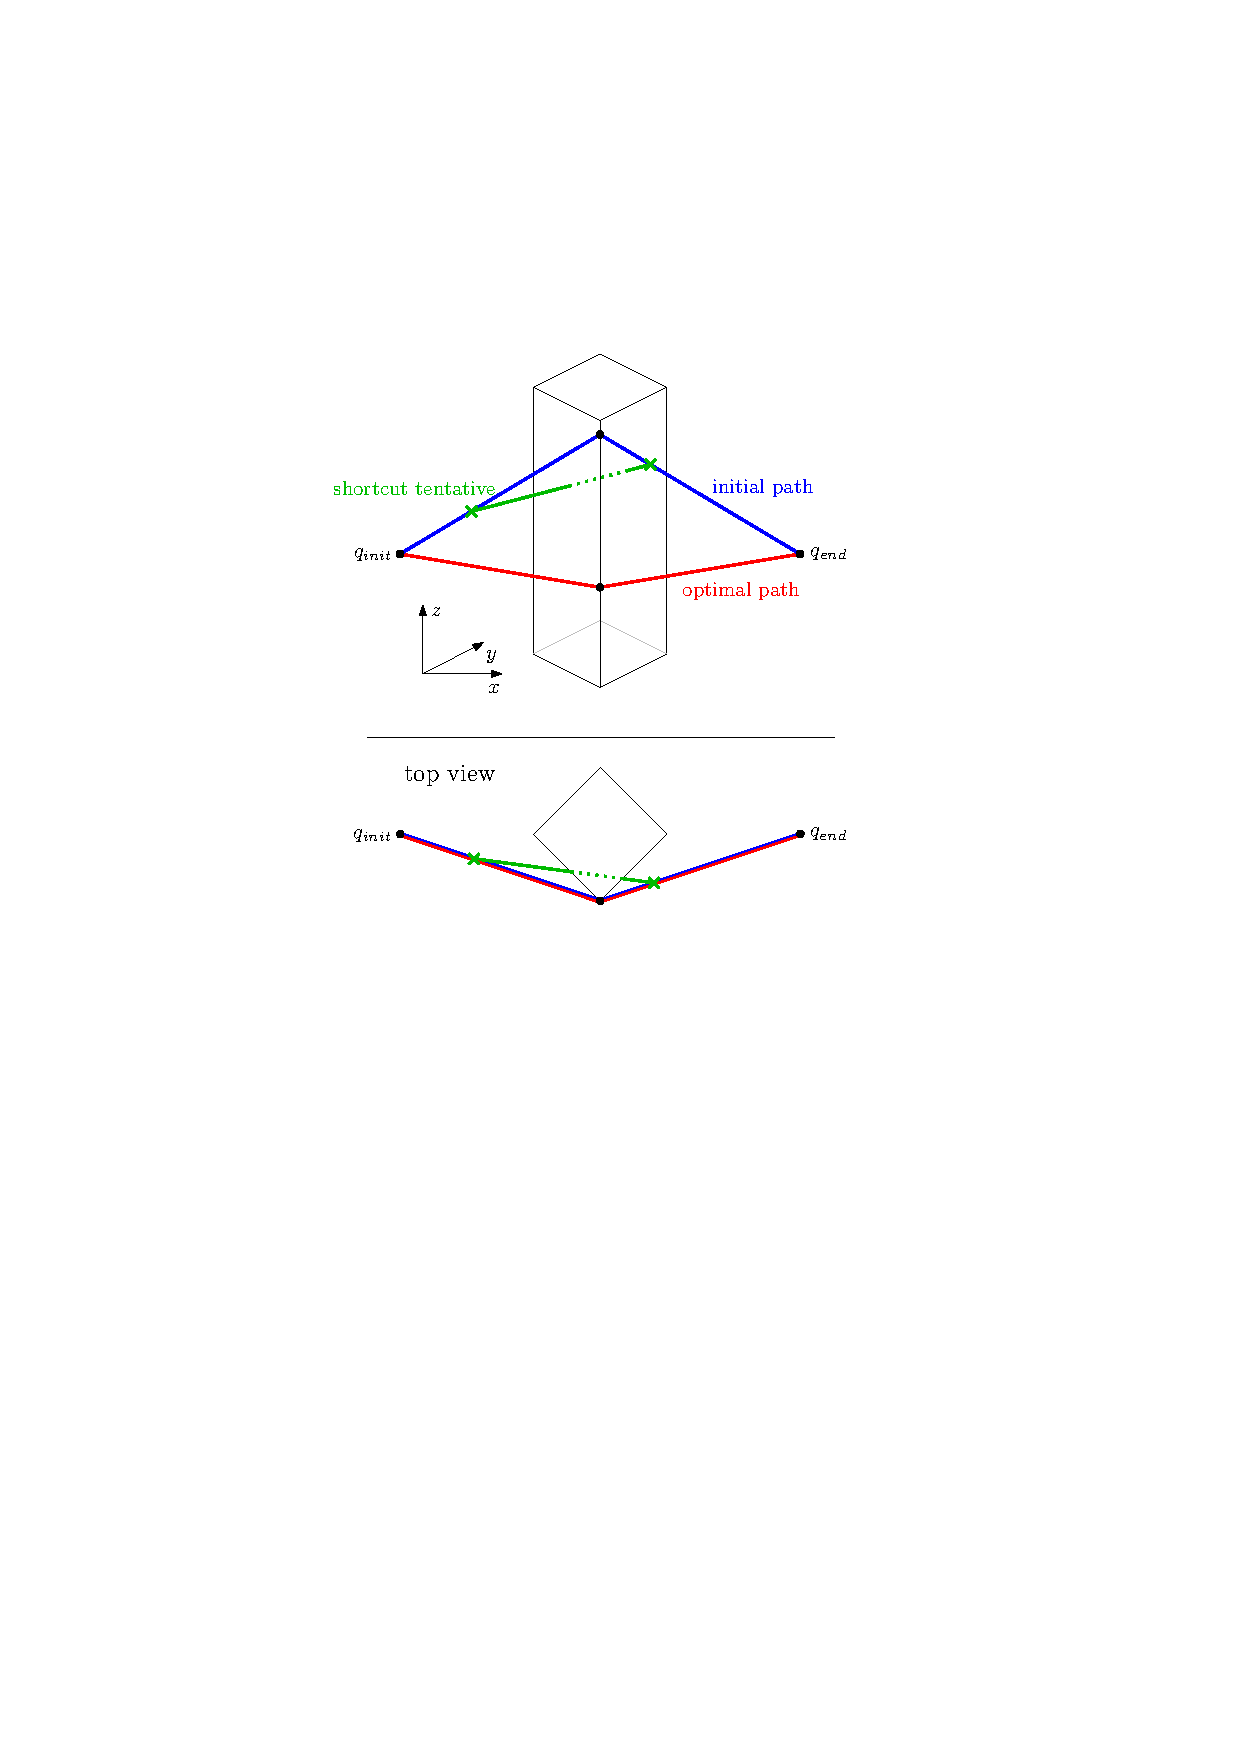
\includegraphics[width=7.5cm]{decoupled_DOF_optimization.pdf}
	\caption{Example of a path which random shortcut will never manage to 
	optimize: each shortcut tentative will provide a collision or will not 
	decrease the path length. The optimal path belongs to the $x-y$ plane 
	containing $q_{init}$ and $q_{end}$.}
	\label{decoupled_DOF_optimization}
\end{figure}


On the other hand, numerical
optimization methods like CHOMP~\cite{RatliffChomp} can be used as a
post-processing step. They have clear termination conditions, but collision
avoidance is handled by inequality constraints sampled at many points along
the trajectory. These methods therefore require a pre-processing step of the
robot (and/or environment) model in order to make 
it simpler:~\cite{RatliffChomp} covers PR2 bodies with spheres, 
while~\cite{convexOptimMotplan} needs to decompose objects into convex subsets.
Moreover, in the applications we address, optimality is not desirable as
such since the shortest path between two configurations in a cluttered
environment usually contains contacts with the obstacle,
or is most of the time
out of the scope of numerical optimization algorithms~\cite{LaumondOptim}.

The idea of our method is to find a good trade-off between
the simplicity of “blind” methods like shortcut algorithm,
and the complexity of distance based optimization techniques.
The method iteratively shortens the initial path with gradient-based information.
When a collision is detected at a given iteration, the method backtracks to the
latest valid iteration and inserts a one-dimensional constraint
between the objects detected in collision. Only collisions between objects are 
evaluated, therefore no pre-processing of the
robot or environment models is necessary to increase distance computation speed. 
Respecting the problem geometry also 
preserves that a solution can still be found, e.g. for narrow passages as holes or 
grippers. The method is also repeatable since no randomness is introduced. The underlying optimization algorithm is a quadratic program.

Related work is presented in Section II. Section III explains how the 
path-optimizer works, from the formulation of the problem to the implemented
algorithm. Finally, we conclude on experimental results in Section IV.

This paper is based on a similar work sent to a conference, where a different type of collision constraints was studied.


\section{RELATED WORK}

CHOMP algorithm~\cite{RatliffChomp} optimizes an initial guess provided as
input. It minimizes a time invariant cost function using efficient covariant
hamiltonian gradient descent. The cost is quantified by non-smooth parts (with
high velocities) and an obstacle avoidance term, provided by the distance to the 
nearest obstacle for each iteration of the trajectory. Calculating these nearest 
distances however is time-consuming because the distances between all pairs of 
objects must be computed at each time step along the path. To reduce the 
computation time, the method starts by building offline a map of distances that 
will be called during the optimization at the requested time. Besides, meshes 
are pre-processed into bounding spheres so that distances are computed faster 
at the cost of a geometry approximation.

STOMP method~\cite{KalakrishnanStomp} avoids to compute an 
explicit gradient for cost optimization using a stochastic analysis of local 
random samples. But as for CHOMP, the obstacle cost term requires a voxel map to 
perform its Euclidian Distance Transforms, and represents the robot bodies with 
overlapping spheres. Such technique provides lots of distance and penetration 
information but remains very time consuming and is not as precise as some 
distance computation techniques based on the problem meshes as 
Gilbert-Johnson-Keerthi~\cite{gilbertGjk}.

Some optimization-based planners may not require an initial guess but some naive 
straight-line manually or randomly-sampled initialization as 
TrajOp~\cite{SchulmanConvexOptim}. Its trajectory is iteratively optimized with 
sequential convex optimization by minimizing at each step its square length, 
linear and non-linear constraints considered as penalties. To compute the 
collision-constraints, nearest obstacle distances are calculated at each discrete 
time of the trajectory vector. This can be a burden for a high-dimensional robot 
or a complex environment as we propose to use, and may be compensated with a 
short path composed of only one or two waypoints.


The elastic strips framework~\cite{BrockElasticStrips} is also an optimization 
based method. The path is modeled as a spring and obstacles give rise to a 
repulsive potential field. Although designed for on-line control purposes, this 
method may be used for path shortening. In this case however, the number of 
distance computation is very high. The authors also proposed to approximate the 
robot geometry by spheres.

Some heuristics use random shortcuts on the initial guess combined with a 
trajectory re-building that returns ${C}^1$ shortcuts made of parabolas and lines 
(bang-bang control)~\cite{HauserFastSmooth}. These local refined trajectories 
are time-optimal since they comply with acceleration and velocity constraints. 
~\cite{Guernane2011}, also based on random shooting, is guiding configuration-
generation with local holonimic considerations. But this method remains only locally 
optimal, and is not addressing high-DOF problems.
~\cite{Geraerts04clearancebased}, whereas just implemented for freeflyer robots, is 
using medial axis retractation for clearance and a PRS (applied only on random DOF) 
which can address the problem of Figure~\ref{decoupled_DOF_optimization} but is 
relatively slower than RS. Moreover, PRS is not using the information returned by 
the checker of which links are colliding to guide which DOF or group of DOF are 
relevant to shortcut, contrary to our method.

In some way, our method shares similarities with~\cite{PanSmoothSplineShort} 
since this latter method relies on collision checking and backtracks when an 
iteration is detected in collision, instead of trying to constantly satisfy 
distance constraints. Unlike our method however, interpolating configuration -which 
can be viewed as constraints- are freezing the whole robot configuration instead of 
a relevant subpart. Thus, this method cannot solve the 
Figure~\ref{decoupled_DOF_optimization} problem.

%Unlike our method however, the iterations are composed of 
%Cubic-B-splines. The benefit of this method is that the result is a 
%differentiable path.



\section{PATH OPTIMIZATION} \label{section:path_optim}

\subsection {Kinematic chain}

A robot is defined by a kinematic chain composed of a tree of joints. We denote 
by $(J_1,\cdots,J_m)$ the ordered list of joints. Each joint $J_i$, $1\leq i\leq 
m$ is represented by a mapping from a sub-manifold of $\real^{n_i}$, where $n_i$ 
is the dimension of $J_i$ in the configuration space, to the space 
of rigid-body motions $SE(3)$. The rigid-body motion is the position of the joint 
in the frame of its parent. In the examples shown in this paper, we consider 4 
types of joints described in Table~\ref{tab:joints}.
\begin{table}[b]
\centerline {
  \begin{tabular}{cccc}
    Name & dimension & config space & velocity\\
    \hline
    translation & 1 & $\real$ & $\real$\\
    bounded rotation & 1& $\real$ & $\real$\\
    unbounded rotation & 2 & $\Sone\subset\real^2$ & $\real$\\
    $SO(3)$ & 4 & $\Sthree\subset\real^4$ & $\real^3$
  \end{tabular}
}
\caption {Translation and rotation joint position are defined by 1 
parameter corresponding respectively to the translation along an axis and a 
rotation angle around an axis. Unbounded rotation is defined by a point on the 
unit circle of the plane: 2 parameters corresponding to the cosine and the 
sine of the rotation angle. $SO(3)$ is defined by a unit quaternion. The 
velocity of translation and unbounded rotation joints is the derivative of the 
configuration variable. The velocity of an unbounded rotation joint corresponds 
to the angular velocity. The velocity of a $SO(3)$ joint is defined by the 
angular velocity vector $\omega\in\real^3$.}
\label{tab:joints}
\end{table}
A configuration of the robot
$$\conf = (\underbrace{q_1,\cdots,q_{n_1}}_{J_1},\underbrace{q_{n_1+1},
\cdots,q_{n_1+n_2}}_{J_2},\cdots q_n),\ n\triangleq\sum_{i=1}^m n_i$$
is defined by the concatenation of the joint configurations. The configuration 
space of the robot is denoted by $\CS\subset\real^n$.

Note that the configuration of the robot belongs to a sub-manifold of $\real^n$.

The velocity of each joint $J_i$, $1\leq i \leq m$ is defined by a vector of $
\real^{p_i}$, where $p_i$ is the number of DOF of $J_i$. Note that 
the velocity vector does not necessarily have the same dimension as the 
configuration vector.

The velocity of the robot is defined as the concatenation of the velocities of 
each joint.
$$\dot{\conf} = (\underbrace{\dot{q}_{1},\cdots,\dot{q}_{p_1}}_{J_1},
\underbrace{\dot{q}_{p_1+1},\cdots,\dot{q}_{p_1+p_2}}_{J_2},\cdots \dot{q}_p),\ p
\triangleq\sum_{i=1}^m p_i$$

\paragraph {Operations on configurations and vectors} by analogy with the case 
where the configuration space is a vector space, we define the following 
operators between configurations and vectors:
$$
\conf_2 - \conf_1 \in \real^p, \ \conf_1, \conf_2\in\CS
$$
is the constant velocity moving from $\conf_1$ to $\conf_2$ in unit time, and
$$
\conf + \dot{\conf}\in\CS, \ \conf\in\CS \ \dot{\conf}\in\real^p
$$
is the configuration reached from $\conf$ after following constant velocity $
\dot{\conf}$ during unit time.

Note that the definitions above stem from the Riemanian structure of the 
configuration space of the robot. The above sum corresponds to the exponential 
map. We do not have enough space in this paper to develop the theory in a more 
rigorous way. The reader can easily state that ``following a 
constant velocity'' makes sense for the four types of joints defined in 
Table~\ref{tab:joints}. We refer to~\cite{riemanian-optim2008} Chapter~5 for 
details about Riemanian geometry.

\subsection {Straight interpolation}

Let $\conf_1, \conf_2\in\CS$ be two configurations. We define the straight 
interpolation between $\conf_1$ and $\conf_2$ as the curve in $\CS$ defined on 
interval $[0,1]$ by:
$$
t \rightarrow \conf_1 + t (\conf_2 - \conf_1)
$$
This interpolation corresponds to the linear interpolation for translation and 
bounded rotations, to the shortest arc on $\Sone$ for unbounded rotation and to 
the so called slerp interpolation for $SO(3)$.

\subsection{Problem definition}

We consider as input a path composed of a concatenation of straight 
interpolations between $wp+2$ configurations: $(\conf_0, \conf_1,\cdots,\conf_{wp
+1})$. This path is the output of a random sampling path planning algorithm 
between $\conf_0$ and $\conf_{wp+1}$. We wish to find a sequence of waypoints $
\conf_{1}$,...,$\conf_{wp}$ such that the new path $(\conf_0, \conf_1,\cdots,
\conf_{wp+1})$ is shorter and collision-free. Note that $\conf_0$ and $\conf_{wp
+1}$ are unchanged and that the workspace of the robot contains obstacles. We 
denote by $\xx$ the optimization variable:
$$
\xx \triangleq (\conf_1,\cdots,\conf_{wp})
$$

\subsubsection {Cost}

let $W\in\real^{p\times p}$ be a diagonal matrix of weights:
$$
W=\left(\begin{array}{cccccccccc}
w_1 I_{p_1}       &        &  0  \\
    & w_2 I_{p_2} &        &   \\
    &            & \ddots &   \\
  0 &            &        & w_m I_{p_m}
\end{array}\right)
$$
where $I_{p_i}$ is the identity matrix of size $p_i$ and $w_i$ is the weight 
associated to the lever arm of the joint $J_i$. We define the length of the straight interpolation 
between two configurations as:
$$
\|\conf_2 - \conf_1\|_{W} \triangleq \sqrt{(\conf_2 - \conf_1)^T W^2 (\conf_2 - 
\conf_1)}.
$$
Weights are used to homogenize translations and rotations in the velocity vector. 
For rotations, the weight is equal to the maximal distance of the robot bodies 
moved by the joint to the center of the joint.

Given $\conf_0$ and $\conf_{wp+1}$ fixed, the cost we want to minimize is defined 
by
$$
\cost (\xx) \triangleq \frac{1}{2}\sum_{i=1}^{wp+1} \lambda_{i-1} \|\conf_{i}-\conf_{i-1}\|_{W}
^{2}
$$
where the $\lambda_{i-1}$ coefficients benefit will be explained in the results 
section. For now we can assume that $\forall i,\, \lambda_{i-1}=1$.

Note that $\cost$ is not exactly the length of the path, but it can be 
established that minimal length paths also minimize $\cost$. This latter cost is 
better conditioned for optimization purposes.

\subsection {Resolution}
We assume that the direct interpolation between the initial and final configurations contains collisions.
Let $H$ denotes the constant Hessian of the cost function, an iteration is 
described as follow:
\begin{equation}\label{eq:iteration-1}
\begin{split}
& \pii =  -H^{-1} \nabla c(\xx_i)^{T} \\
& \xx_{i+1} =  \xx_{i} + \alpha_i \pii
\end{split} 
\end{equation}
where $\alpha_i$ is a real valued parameter. Taking $\alpha_i=1$ yields the 
unconstrained minimal cost path, i.e. all waypoints aligned on the straight line 
between $q_0$ and $q_{n+1}$. Since this solution is in collision, we set 
$\alpha_i = \alpha$ 
where $\alpha$ is a parameter that will be explained in the algorithm section.

We iterate step~(\ref{eq:iteration-1}) until path $\xx_{i+1}$ is in collision. This 
corresponds to the unconstrained function \texttt{computeIterate} in 
Algorithm~\ref{algo:gradient}.
When a collision is detected, we introduce a constraint and perform a new 
iteration from $\xx_i$ as explained in the next section. We use a continuous 
collision checker inspired of~\cite{SchwarzerExactCollision} to validate our 
paths and to return the first colliding configuration along a path. This step corresponds to \texttt{validatePath} in Algorithm~\ref{algo:gradient}.

\subsection{Constraints}

\begin{figure}[t]
	\centering
	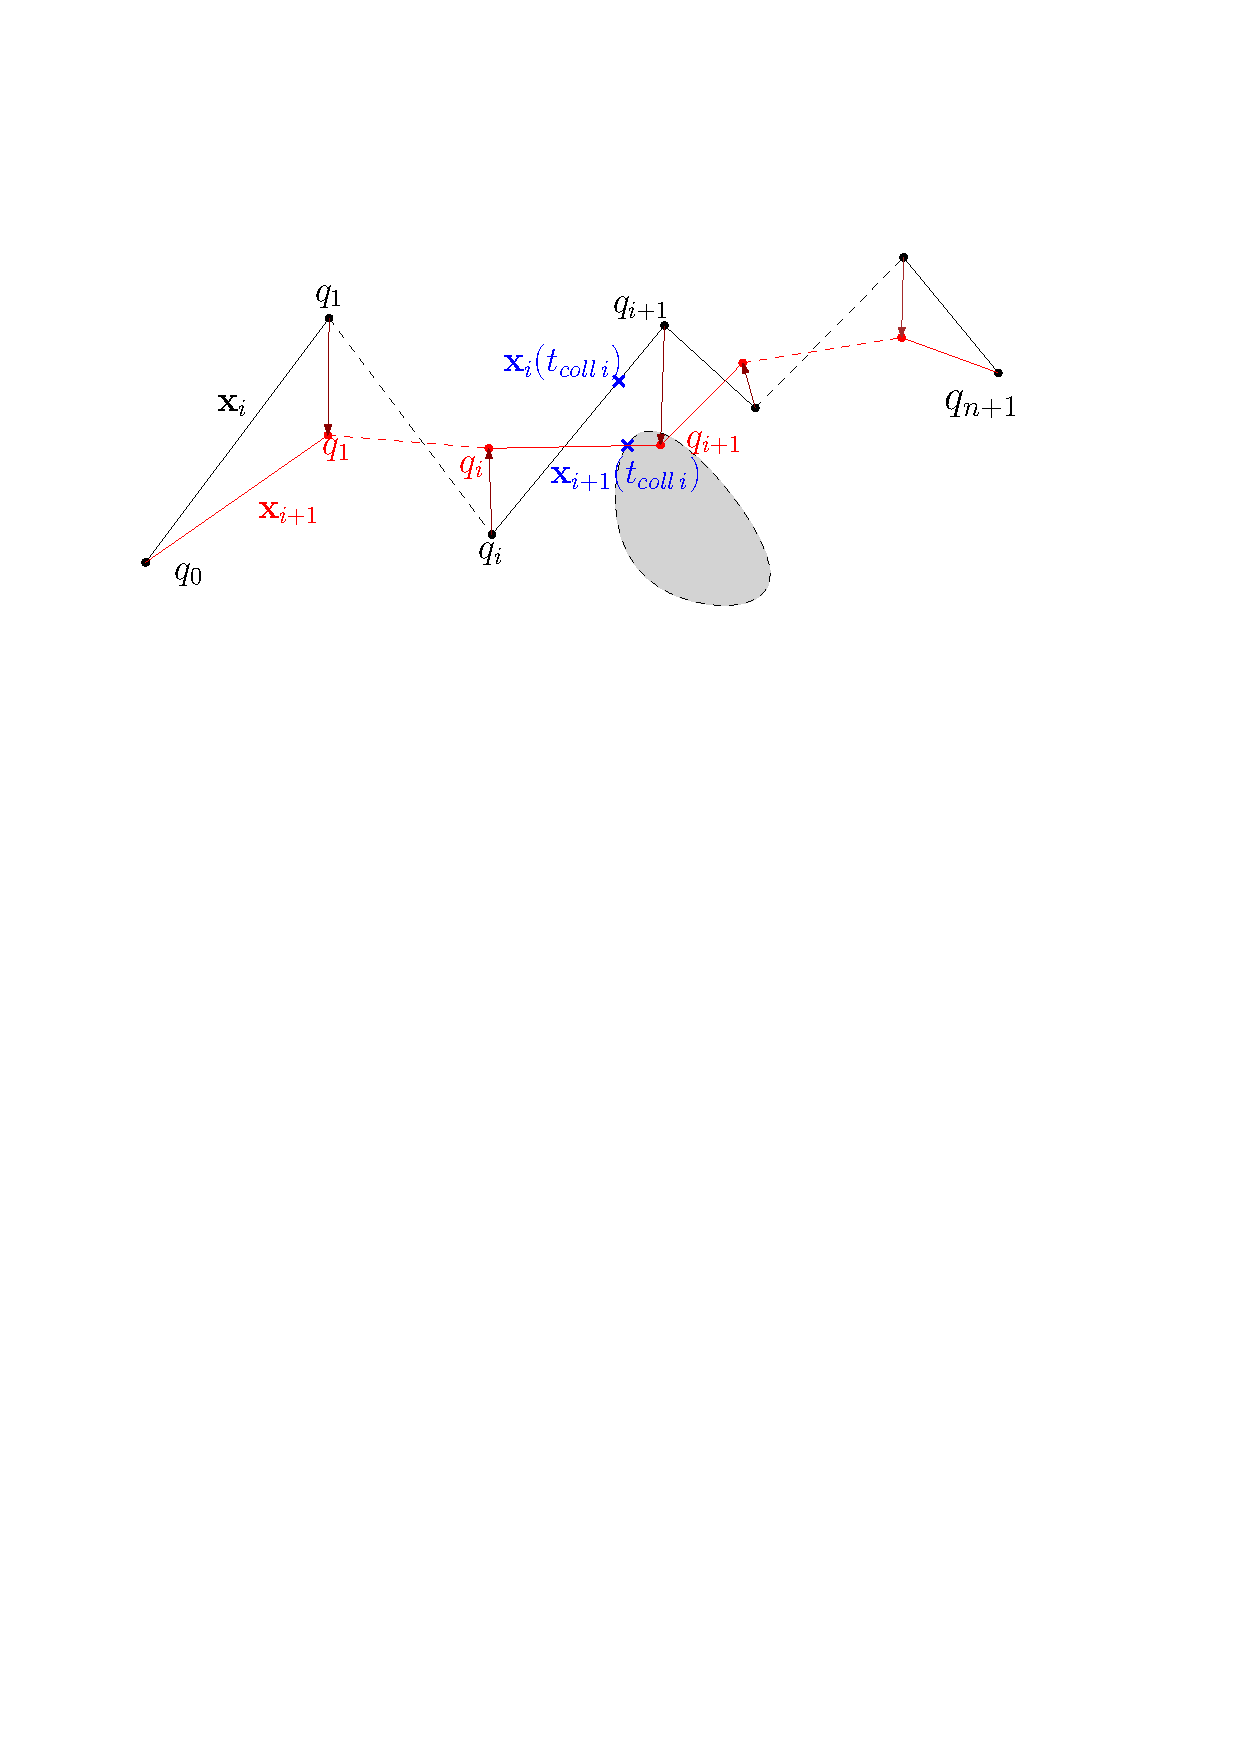
\includegraphics[width=9cm]{optim_grad.pdf}
	\caption{Illustration of one iteration of our optimization. $\xx_{i+1}$ 
	appears 
	to be in collision with the obstacle, the first colliding configuration 
	$\xx_{i+1}(\tcolli)$ is returned by the continuous collision checker. The corresponding constraint will be computed in configuration $\xx_{i}(\tcolli)$.}
	\label{optim_grad}
\end{figure}

Let us assume that at iteration $i$, $k$ constraints have been inserted before the current interation. These constraints are stored as lines of a Jacobian matrix
$$
\Jf_{i} = \left(\begin{array}{c}L_1 \\ \vdots \\ L_k\end{array}\right)
$$
where iterate $\p_i$ are constrained to be in the kernel of $\Jf_{i}$
$$
\Jf_{i} \p_i = 0
$$

\subsection*{New constraint}

Let $T$ be a positive real number such that each path $\xx_i$ is a mapping from 
interval $[0,T]$ into $\CS$: $\xx_i(0) = q_0$, $\xx_i(T) = q_{n+1}$ for all $i$. Let 
us denote by $\tcolli$ the abscissa of the first collision detected on path 
$\xx_{i+1}$, which previous iteration $\xx_i$ was collision-free (see 
Figure~\ref{optim_grad}). Thus in 
configuration $\xx_{i+1}(\tcolli)$ a collision has been 
detected. Two cases are possible:
\begin{enumerate}
\item the collision occurred between two bodies of the robot: $\body_1$ and $
\body_2$, or
\item the collision occurred between a body of the robot $\body_1$ and the 
environment.
\end{enumerate}
In the rest of this section, we will only consider the first case. Reasoning 
about the second case is similar, except that the 
constraint is on the position of $\body_1$ with respect to the environment.

\begin{figure}[t]
	\centering
	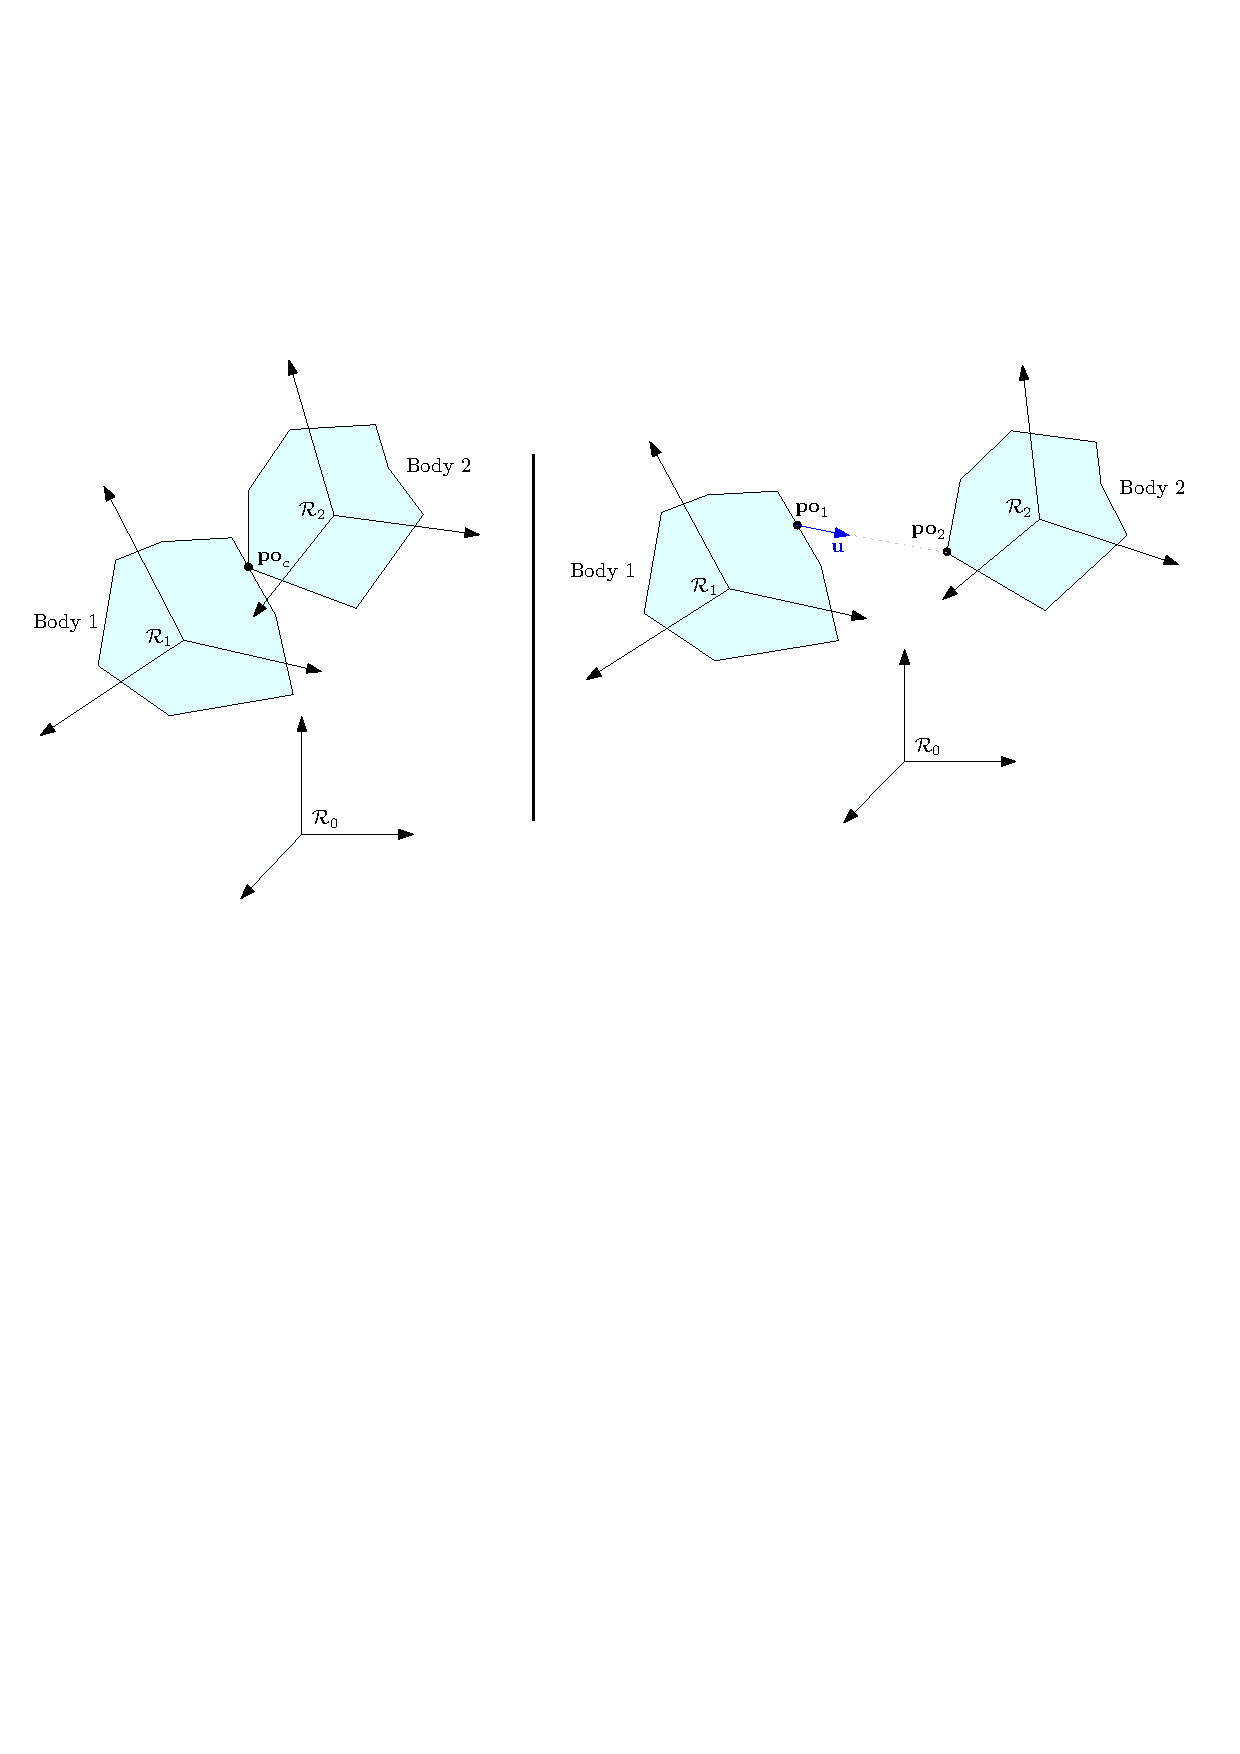
\includegraphics[width=15.8cm]{contact-points.pdf}
	\caption{Bodies representation in collision-configuration (left) and 
	backtracked free-configuration (right). A contact point (i.e. any point in 
	the intersection of the bodies) $\po_c$ can be returned by the Flexible 
	Collision Library~\cite{fcl}, used to detect collisions. The red $(\perp)$ 
	hyperplan is orthogonal to ($\po_2$,$\mathbf{u}$) and represents the motion 
	direction which is allowed by the constraint.}
	\label{contact-points}
\end{figure}

The principle of the method is to compute a constraint on the backtracked free-
configuration $\xx_{i}(\tcolli)$ to avoid the encountered collision $\xx_{i+1}
(\tcolli)$. To handle this, we introduce a one-dimensional constraint based on the 
orthogonal direction of the encountered collision.

In the collision-configuration $\xx_{i+1}(\tcolli)$, let $\po_c\in \real^3$ be a 
contact point expressed in the global frame ${\cal R}_0$ 
(Figure~\ref{contact-points} left). We compute the respective positions $\po_1$ and 
$\po_2$ of $\po_c$ in 
the local frames of $\body_1$ and $\body_2$ (Figure~\ref{contact-points} right).

Let $M_1 \in SE(3)$ (resp. $M_2 \in SE(3)$) denote the homogeneous transformation 
between frames of $\body_1$ (resp. $\body_2$) and the global frame in configuration 
$\xx_i(\tcolli)$. Let $\mathbf{u}$ be the unit vector 
linking the contact points in configuration 
$\xx_{i}(t_{coll\ i})$ (the latest collision-free path), expressed in the local 
frame of $\body_1$:
$$
\mathbf{u} = \frac{M_{1}^{-1} (\xx_i) M_2 (\xx_i) \po_2 - \po_1}{\|M_{1}^{-1} 
(\xx_i) M_2 (\xx_i) \po_2 - \po_1\|}
$$

Notice that $\mathbf{u}$ is well defined since configuration 
$\xx_{i}(t_{coll\ i})$ is collision-free.
Let $f$ be the function defined from $\CS^{wp}$ to $\real$ by:
$$
f (\xx) = \left(M_{1}^{-1} (\xx) M_2 (\xx) \po_2 - \po_1 | \mathbf{u}\right)
$$
The constraint is defined by
\begin {equation}\label{eq:new-constraint}
f(\xx) - f(\xx_{i}) = 0.
\end {equation}
As this constraint is non-linear, it is linearized around $\xx_{i}$.

Let $q_{k\,i}$ denote the waypoint $k$ along path $x_i$.
The constraint on the position at $t_{coll\,i}$ is a function that depends only
on two waypoints $q_{k\,i}$, $q_{k+1\,i}$, with $0\leq k\leq n$. There exists 
$\beta\in[0,1]$ such that for any $j$:
$$
\xx_j (t_{coll\,i}) = \conf_{k\,j} + \beta (\conf_{k+1\,j} - \conf_{k\,j})
$$
The path Jacobian $\frac{\partial f}{\partial \xx}(\xx_i)$ is thus built by matrix 
blocks using the previous constraint Jacobian $\frac{\partial f}{\partial \conf}$ 
and $\beta$, corresponding to \texttt{computeCollisionConstraint} in 
Algorithm~\ref{algo:gradient}.
Then, a line is added in the contraint Jacobian matrix (function 
\texttt{addCollisionConstraint}), and the constraint 
Jacobian becomes:
\begin {align*}
\Jf_{i+1} &= \left(\begin{array}{c}L_1 \\ \vdots \\ L_{k+1}\end{array}\right)\ \mbox {with}\\
L_{k+1} &= \frac{\partial f}{\partial \xx}(\xx_i)
\end{align*}



%Let $\translation^{*}\in \real^3$ denotes the position between frames of $
%\body_1$  and $\body_2$ in configuration $\xx_i(\tcolli)$. Let $\translation \in 
%\real^3$ (resp. $R\in SO(3)$) denote the same position (resp. rotation) in 
%configuration $\xx (\tcolli)$ where $\xx$ is any path in $\CS^{wp}$.

%Let $M^{*}\in SE(3)$ denote the homogeneous transformation between frames of $
%\body_1$  and $\body_2$ in configuration 
%$\xx_i(\tcolli)$. Let $M\in SE(3)$ denote the same transformation in configuration 
%$\xx (\tcolli)$ where $\xx$ is any path 
%in $\CS^{wp}$. Let $R\in SO(3)$ and $\translation\in\real^3$ 
%(resp. $\translation^{*}$) be the rotation 
%and translation parts of $M$ (resp. $M^{*}$).

%We denote by $F$ the path constraint defined by the mapping from $\CS^{wp}$ to $
%\real^3$ defined by
%\begin{equation}\label{eq:constraint}
%F (\xx) =  \mathbf{u}^T R^T (\translation^{*} - \translation)
%\end{equation}
%where the product $R^T (\translation^{*} - \translation)$ is used to express the translations difference in the global frame ${\cal R}_0$.

\vspace{0.2cm}


%Therefore, the Jacobian $J_F$ of constraint~(\ref{eq:constraint}) with respect to 
%$x$ is
%$$
%J_F = \left(\begin{array}{cccccc}
%0 & \cdots & (1-\beta)\,\mathbf{u}^T \frac{\partial F}{\partial q} (\xx_j(t_{coll\,i})) & \
%\beta\,\mathbf{u}^T \frac{\partial F}{\partial q} (\xx_j(t_{coll\,i})) & \cdots & 0
%\end{array}
%\right)
%$$


\vspace{0.2cm}

Then we refer to~\cite{nocedal2006numerical} for solving constrained quadratic 
programs (QP) (function \texttt{computeIterate} in 
Algorithm~\ref{algo:gradient}).

%The solution step is given by:
%$$
%\mathbf{\pii}^{*} = -V_0(V_0^TH V_0)^{-1}\,V_0^T\nabla c(\xx_i)
%$$
%where $V_0$ is the base of the nullspace of the stack of $J_F$ jacobians.


\subsection*{Convergence Analysis}
For iteratively constrained problem, the risk of falling in an infinite loop 
that keeps adding a redundant constraint exists.
In this section, we demonstrate that, given the constraint definition and the 
function \texttt{solveRedundantConstraint}, our 
algorithm will converge.
Under the previous notations, it is straight-forward that
\begin{equation}\label{eq:decreasing-kernel}
\kernel \Jf_{i+1} \subset \kernel \Jf_{i}
\end{equation}
Let us assume that
\begin{equation}\label{eq:asumption-1}
L_{k+1}\p_i \not= 0.
\end{equation}
We will elaborate later on this asumption. This means that $\p_{i}\notin\kernel J_{i+1}$, and as $\p_{i}\in\kernel J_{i}$, then
$$
\kernel J_i \not= \kernel J_{i+1}.
$$
From~(\ref{eq:decreasing-kernel}), we deduce that
$$
\dim (\kernel J_{i+1}) < \dim (\kernel J_i).
$$
This results proves that each added constraint is linearly independant from the 
previous ones, and thus our algorithm terminates in a finite number of iterations.

\subsubsection*{About asumption~(\ref{eq:asumption-1})}%
Let us consider the following expression:
$$
\frac{\partial f}{\partial \xx}(\xx_{i+1})\p_i
$$
This expression represents the velocity of point $\po_2$ in the reference frame of Body~1 projected onto $\mathbf{u}$ along the motion of the robot defined by the following trajectory:
\begin{equation}\label{eq:trajectory}
\conf (t) = \xx_{i}(t_{coll\ i}) + t\, \alpha_i \p_{i}.
\end{equation}
The motion is defined by taking a constant abscissa $t_{coll\ i}$ and be moving the 
path along iterate $\p_i$. Note that configuration $\xx_{i+1}(t_{coll\ i})$ is 
reached for $t=1$.
This expression being equal to 0 requires either
\begin {enumerate}
\item that $\po_1$ and $\po_2$ come to contact at zero velocity, or
\item the velocity of $\po_2$ in the reference frame of Body~1 is orthogonal to 
$\mathbf{u}$ at contact ($t=1$).
\end {enumerate}
The first case is very unlikely and almost never encountered in real applications, 
except if the user builds such a case on purpose.
The second case may appear and can be noted by a rank loss of $\Jf_{i+1}$. In this 
case, we do not directly insert the new constraint. Instead, we process intermediate 
iterations until the redundancy vanishes, as explained in function 
\texttt{solveRedundantConstraint}.

\begin{algorithm}
\begin{algorithmic}%[1] % line numerotation
\INPUT{$\xx_{Free}$ latest collision-free path, $\xx_{Coll}$ current path with collisions, $\p$ current iteration step}
\Require constraint $\frac{\partial f}{\partial \xx} (\xx_{Free})$ built from $\xx_{Coll}$ would produce a rank loss in constraint Jacobian $\Jf$
\State $solved \gets false$
\State $minReached \gets false$
\While{($\textbf{not}(solved)$)}
	\State $\p = \texttt{computeIterate}()$
	\State $minReached = (||\p||<10^{-3} \textbf{ or } \alpha=1)$
	\State $\xx \gets \xx_{Free} + \frac{\alpha}{2}\,\p$
	\If{(\texttt{validatePath}($\xx_1$))}
		\State $\xx_{Free} \gets \xx$
	\Else
		\State $\xx_{Coll} \gets \xx$
	\EndIf
	\State $\frac{\partial f}{\partial \xx} (\xx_{Free}) \gets$\texttt{computeCollisionConstraint}($\xx_{Coll}$, $\xx_{Free}$)
	\State $solved \gets$ \texttt{isFullRank}($\Jf$ , $\frac{\partial f}{\partial \xx} (\xx_{Free})$)
\EndWhile
\end{algorithmic}
\caption{\texttt{solveRedundantConstraint}()} \label{algo:solveRedundant}
\end{algorithm}

After producing an intermediate iteration $\xx_{i+2}$ where $\alpha_i$ was 
halved, the obtained path is tested for collisions. If it is collision-free, the 
constraint is now linearized around it. Otherwise, new contact points are taken 
on it, and the constraint is linearized around the latest free path.

Doing so, either the new constraint makes the dimension of the kernel decrease, or 
makes the configuration in collision ($\xx_{i+1}$ or $\xx_{i+2}$ depending on the 
case above) and the latest collision-free path ($\xx_{i}$ or $\xx_{i+2}$) become 
closer and closer. And the continuity of $f$ implies that
$$
\frac{\partial f}{\partial \xx}(\xx_i)\p_i \ \ \ \mbox{and}\ \ \ \frac{\partial f}{\partial \xx}(\xx_{i+1})\p_i
$$
converge toward the norm of the velocity of point $\po_2$ in the reference frame of 
body~1 along trajectory~(\ref{eq:trajectory}) when $\po_2$ and $\po_1$ come to 
contact. We already handled this case previously, admitting that the velocity norm 
would not vanish. Therefore, is~\ref{eq:asumption-1} verified.



\subsection{Algorithm}

In this part we describe the GB path-optimizer Algorithm~\ref{algo:gradient} 
according to the previous step definitions. The main difficulty here is to handle 
the scalar parameter $\alpha$ determining how much of the computed step $\p$ will 
be traveled through, and also to return a collision-free path. Typically, we 
chose $\alpha_{init} = 0.2$ or 0.1 to process small steps. $\alpha_{init} = 0.5$ is 
more encountered in the optimization literature, procuring larger steps but with 
more risks of collision.

\begin{algorithm}
\begin{algorithmic}%[1] % line numerotation
\INPUT{Path to optimize $\xx_0$}
\OUTPUT{Optimized collision-free path $\xx_0$}
\State $\alpha \gets \alpha_{init}$
\State $minReached \gets false$
\While{($\textbf{not}(noCollision \textbf{ and } minReached)$)}
	\State $\p = \texttt{computeIterate}()$
	\State $minReached = (||\p||<10^{-3} \textbf{ or } \alpha=1)$
	\State $\xx_1 \gets \xx_0 + \alpha\,\p$
	\If{(\textbf{not}(\texttt{validatePath($\xx_1$)}))}
		\State $noCollision \gets false$
		\If{$(\alpha \neq 1)$}
			\State \texttt{computeCollisionConstraint}($\xx_1$, $\xx_0$)
			\State \texttt{solveRedundantConstraint}()
			\State \texttt{addCollisionConstraint}()
			\State $\alpha \gets 1$
		\Else
			\State $\alpha \gets \alpha_{init}$
		\EndIf
	\Else
		\State $\xx_0 \gets \xx_1$
		\State $noCollision \gets true$
	\EndIf
\EndWhile
\end{algorithmic}
\caption{Gradient-based (GB) algorithm for path-optimization.} \label{algo:gradient}
\end{algorithm}

Each time a collision-constraint is added, 
the solution of the current QP is tested (i.e. $\alpha = 1$). If this path is collision-free, the algorithm returns it as the solution. Otherwise, 
smaller steps are iteratively applied and tested toward the minimum, and constraints are added each time a collision is found with a small step (i.e. $\alpha \neq 1$).


\section{RESULTS}

This part gathers optimization results performed on the planning software 
Humanoid Path Planner~\cite{hpp}. The initial trajectory is obtained with two 
kind of probabilistic planners: Visibility-PRM~\cite{visibility-prm} and 
RRT-connect~\cite{rrt-connect}.

\subsection{From 2D basic examples...}

\begin{figure}[t]
	\centering
	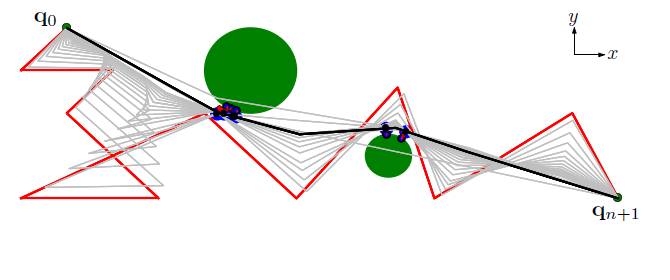
\includegraphics[width=7.8cm]{contact_points6.png}
	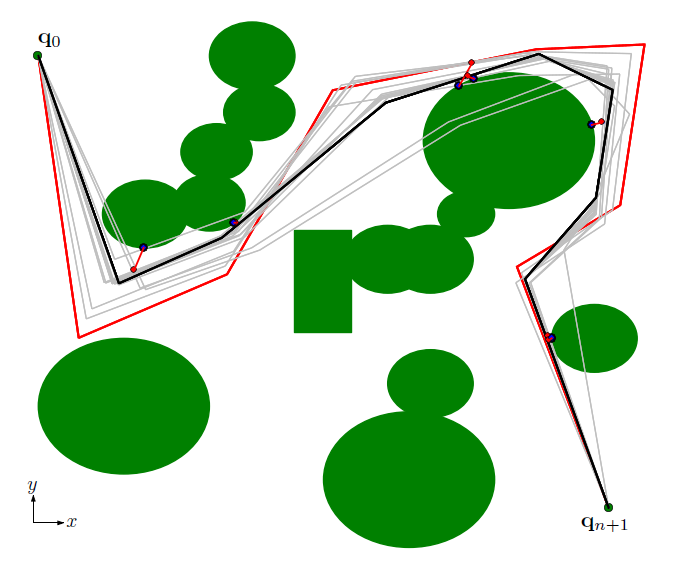
\includegraphics[width=8cm]{contact_points2potential.png}
	\caption{Path-optimization results on 2D-ponctual robots, moving around 
	green obstacles. Initial paths are in red, optimized ones in black. Grey paths 
	represent intermediate iterations, red and black dots resp. $\po_1$ and $\po_2$ 
	points, red segments $\mathbf{u}$ and blue circles collision-free 
	configurations 
	of the backtracked paths 
	where constraints have been computed.}
	\label{2D_long}
\end{figure}

Figure~\ref{2D_long} shows several iterations of our optimizer on 2D cases. Since 
in this special case, orthogonal constraints are equivalent to forbidden motion 
direction, we can verify that our optimized path is applying 
all computed constraints. We can also understand which collisions have led to 
the constraints.

Besides, these examples give a better understanding of how the tuning of $\alpha$ 
has to balance lot of iterations and relevant collision-constraint addition. For 
example, if we alter a lot the initial path with a large gradient step and 
compute the corresponding collisions, constraints will be chosen on a very-not 
optimal path and will not be pertinent w.r.t. the obstacles we wanted to 
avoid.

Figure~\ref{local_box_optim} illustrates a \textit{very long} path example that RS 
or PRS will not manage to 
optimize in an affordable time, because of probabilistically failing to sample 
configurations in the box. GB succeeds to optimize the 
path contained in the box, with the following cost coefficients 
$$
\lambda_{i-1} = \frac{1}{\sqrt{(\conf_{i\,0}-\conf_{i-1\,0})^T \weight^2 
(\conf_{i\,0}-\conf_{i-1\,0})}}
$$
aiming at keeping the same ratio between path segment lengths at 
minimum as at 
initial path, represented by the waypoints ($\conf_{i\,0})_{1\leq i\leq n+1}$.
Without these coefficients, the path that minimizes the cost corresponds to a 
straight line with the waypoints equidistantly allocated, which is not adapted for 
the Figure~\ref{local_box_optim} type of problems with a local passage very
constrained by obstacles. Note that this cost is also working with all other 
examples presented in this paper.


\begin{figure}[t]
	\centering
	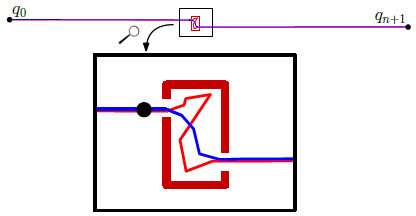
\includegraphics[width=7.5cm]{local_box_optim.png}
	\caption{Case of a long initial path (above) containing a small part that can 
	be optimized (below). Random shortcut is unlikely to optimize the part 
	containing detours in the box, whereas our method 
	succeeds (in blue). This type of issue is common in navigation problems in 
	environments with long corridors.}
	\label{local_box_optim}
\end{figure}



\subsection{To 3D complex problems}

We also experiment our algorithm on more complex robots, with transformation 
collision-constraints. Unless another value is given, $\alpha_{init}$ is set to 0.2.

%\begin{figure}[b]
%	\centering
%	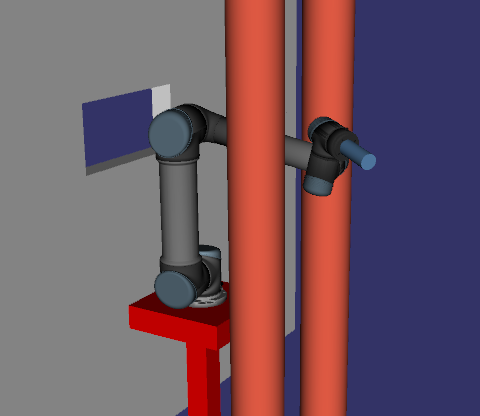
\includegraphics[width=5cm,height=3.5cm]{ur5_v2.png}
%	\caption{6-DOF robot arm on which our path-optimization has been tested.}
%	\label{ur5}
%\end{figure}


\begin{algorithm}
\begin{algorithmic}[1] % line numerotation
\Procedure{randomShortcut}{$\xx$}
   \State nbFailures $\gets 0$
   \While {$nbFailures < maxNbFailures$}
        \State $failure \gets true$
        \State $T \gets \mbox{upper bound of }\xx\mbox{ definition interval}$
        \State $t_1 < t_2 \gets \mbox{random numbers in }[0,T]$
        \State $lp0 \gets \texttt{steeringMethod} (\xx(0), \xx(t_1))$
        \State $lp1 \gets \texttt{steeringMethod} (\xx(t_1), \xx(t_2))$
        \State $lp2 \gets \texttt{steeringMethod} (\xx(t_2), \xx(T))$
        \State $newPath \gets \mbox{empty path defined on }[0,0]$
   	\If{$lp0$ is collision-free}
          \State $newPath \gets lp0$; $failure \gets false$
        \Else
          \State $newPath \gets \xx_{|[0,t_1]}$
        \EndIf
   	\If{$lp1$ is collision-free}
          \State $newPath \gets \texttt{concatenate} (newPath, lp1)$
          \State $failure \gets false$
        \Else
          \State $newPath \gets \texttt{concatenate} (newPath, \xx_{|[t_1,t_2]})$
        \EndIf
   	\If{$lp2$ is collision-free}
          \State $newPath \gets \texttt{concatenate} (newPath, lp2)$
          \State $failure \gets false$
        \Else
          \State $newPath \gets \texttt{concatenate} (newPath, \xx_{|[t_2,T]})$
        \EndIf
        \State $\xx \gets newPath$
        \If {$failure$} $nbFailures \gets nbFailures + 1$
        \EndIf
      \EndWhile
    \Return $\xx$
\EndProcedure
\end{algorithmic}
\caption{Random shortcut as adapted from~\cite{Sekhavat-Svestka1998} 
Section~6.4.1. \texttt{steeringMethod} returns the linear interpolation between 
two configurations. $\xx_{|I}$ denotes path $\xx$ restricted to interval $I$. 
$maxNbFailures$ is a parameter that affects time of computation and quality of 
the result.}\label{algo:random-shortcut}
\end{algorithm}

\begin{figure}[b]
	\centering
	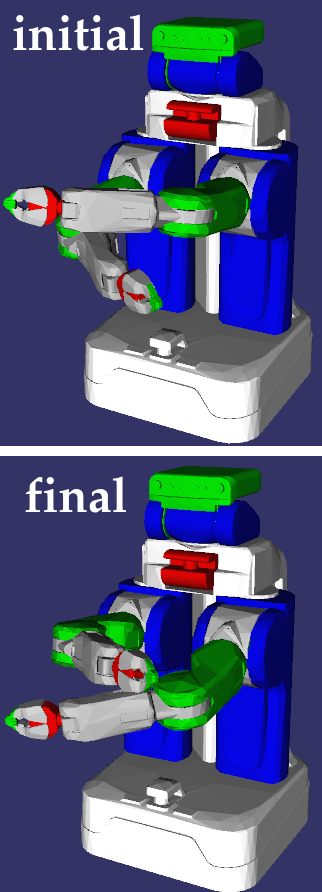
\includegraphics[height=4.9cm,width=1.8cm]{pr2_initial_final_vertical.png}
	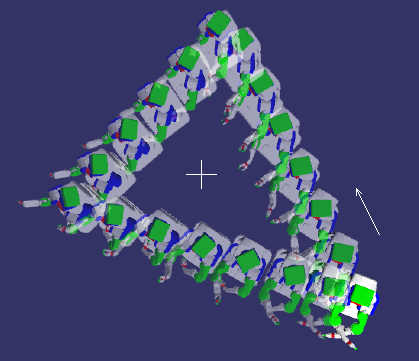
\includegraphics[width=5.7cm]{p0_pr2_alone_merged3.png}
	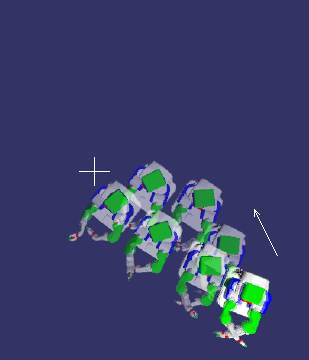
\includegraphics[height=4.9cm]{p1RS_pr2_alone_merged3.png}
	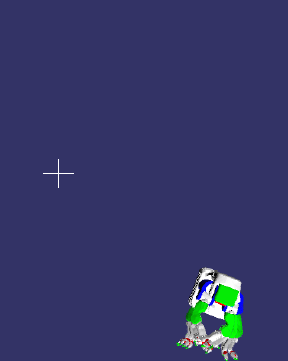
\includegraphics[height=4.9cm]{p1GB_pr2_alone_merged3.png}\\
	\caption{PR2-crossing-arms example. In this motion planning problem, PR2 robot 
	has just to 
exchange the positions of its arms. The task is simple, however, in absence of 
explicit indication, any probabilistic motion planner will compute a path that 
makes the PR2 mobile base purposelessly moving. This is the case of RRT-connect 
algorithm (left). Path optimization is expected to remove unnecessary motions. 
The popular RS algorithm fails in this case (middle). Our GB algorithm 
succeeds (right).}
	\label{pr2_final}
\end{figure}

In the included video and Figures~\ref{pr2_final},~\ref{fiad} and
 ~\ref{fig:trajectories}, we present multiple situations where the GB algorithm has 
been tested and compared to RS~\cite{randomShortcutHPP}
(Algorithm~\ref{algo:random-shortcut}) and PRS ~\cite{partialrandomShortcutHPP} 
adapted from~\cite{Geraerts04clearancebased}.
The termination condition of RS allows it to try 
shortening the path until 5 iterations of non-improvement are reached 
(corresponding to $maxNbFailures$ in Algorithm~\ref{algo:random-shortcut}).
For our implementation of PRS, first a shortcut is tried on each DOF between 
$\conf_0$ and $\conf_{n+1}$. 
Then, for each DOF, configurations are shot as in 
Algorithm~\ref{algo:random-shortcut} and the steering-method returns a path made by 
an interpolation on only 
the current DOF and the previous subpath for other DOF. If this path is collision-
free, it is replaced as in RS. This process is also stopped when 5 iterations of 
non-improvement are reached.

%But we admit that restrincting the number of random shortcut iterations is 
%neither a acceptable criterion because of randomness.
%We also discuss the good properties and limits of our algorithm.

\vspace{0.4cm}
% freeflyer puzzle
Before entering the manipulators examples, the GB algorithm is tested and compared 
on a freeflyer puzzle example (see Figure~\ref{fig:trajectories} top right), very 
encountered in the motion planning literature. The puzzle has to cross down the 
obstacle using the hole in the middle. The initial path planned with Visibility-PRM 
contains detours above and below the obstacle, as well as small motion in the hole. 
Lengths of initial, GB optimized, and RS optimized paths are 
respectively 23.4, 8.53 and 10.2. PRS fails to decrease the path length because in this problem, all DOF are closely related to cross the hole. This behaviour was also noticed and improve in the PRS implementation of~\cite{Geraerts04clearancebased}, acting on a group of DOF. The GB optimizer manages to modify the puzzle trajectory even in the hole, contrary to RS which simply copies the initial path when the trajectory gets near of the obstacle.

\vspace{0.4cm}

% double-arm:
On the double-arm problem (see Figure~\ref{fig:trajectories} top-left), one arm has 
to get around a cylinder obstacle while the 
other arm is relatively far from obstacles. As expected, the initial path given by 
RRT-connect activates both arms to solve the problem. Contrary to RS, 
GB manages to cancel the rotation of the free-arm while optimizing the 
first arm motion, even if the second arm is still moving because of the translation 
motion. The initial path length 5.17 is decreased to 4.55 by RS, to 4.06 by PRS and 
to 2.77 by GB using 3 collision-constraints with the cylinder obstacle.


\begin{figure}[t]
	\centering
	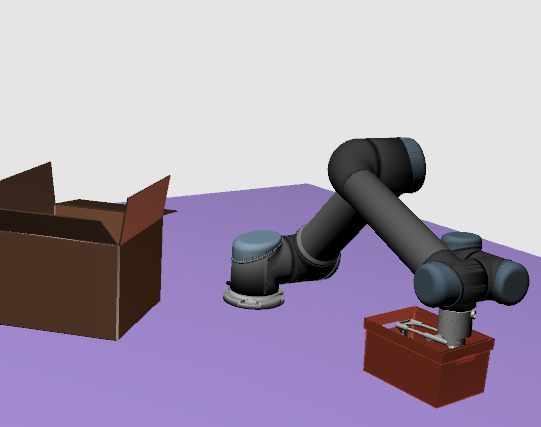
\includegraphics[width=5.8cm,height=4.7cm]{fiad_qinit.png}
	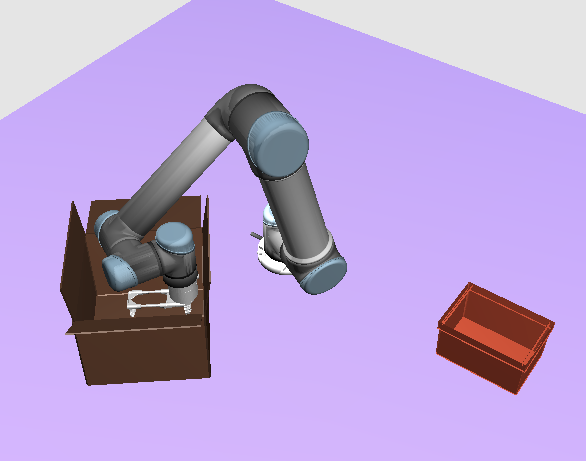
\includegraphics[width=5.8cm,height=4.7cm]{fiad_qfinal.png}\\
	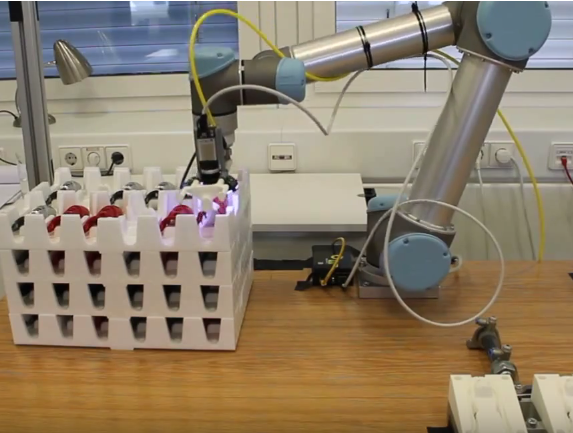
\includegraphics[width=5.8cm,height=4.7cm]{fiad_real.png}
	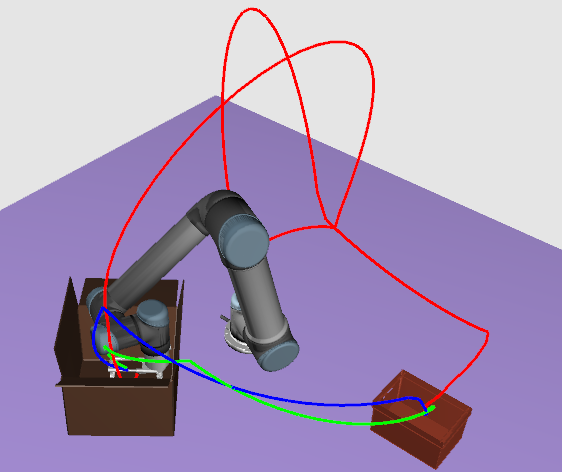
\includegraphics[width=5.8cm,height=4.7cm]{fiad-trajectorires.png}
	\caption{(Bottom left) An industrial use-case example proposed by Philips for 	
	the Factory-in-a-Day project~\cite{factory-day-video}. A similar environment 	
	has been created (top) to illustrate that our method can comply with an 
	industrial problem, where initial and final configurations of the UR5 are 
	constrained in boxes. Trajectories results 
	are presented (bottom right): initial (RRT) path in red, RS optimization in 
	blue and GB optimization in green.}
	\label{fiad}
\end{figure}

% UR5-spheres:
Some problems were 
involving an a 6-axis manipulator arm, also called UR5, equipped with a bar or a 
gripper.
In a relatively free environment (Figure~\ref{fig:trajectories} middle right), 
results from GB and RS are similar (path length are respectively 2.03 and 1.60). 
Note also that the end-effector trajectory has completely changed from the initial 
one, the robot is easily passing between the spheres, keeping its end-effector 
above.

% UR5-fiad
For an UR5 working in a cluttered environment inspired from an industrial issue 
Figure~\ref{fiad}, path optimization efficiently returns a shorter solution, close 
to the result of RS and to what can be observed in reality~\cite{factory-day-video}. 
The initial path length 6.65 is decreased to 2.08 by RS, to 
1.98 by GB and unchanged by PRS.

% UR5-wall  OPTIONAL PART imo
%\begin{wrapfigure}[16]{r}{7cm}
%\centering
%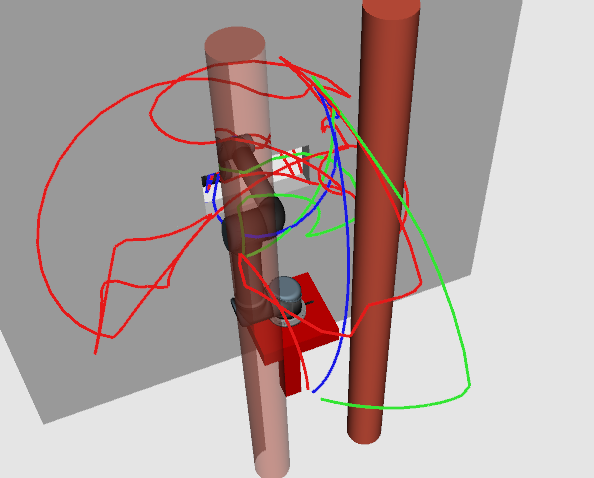
\includegraphics[width=7cm]{ur5-wall-traj-rank-loss.png}
%\caption{UR5}
%\label{ur5-wall}
%\end{wrapfigure}
%In a much more cluttered environment Figure~\ref{ur5-wall} where the robot moves 
%throught a hole in a wall and between two cylinders, path reduction only manages to 
%reduce some but not 
%all detours. This behavior can be explained by a path over-constraining due to the 
%important proximity of the robot to the obstacles during the whole path, and 
%because there are not so many DOF to play on to easily avoid collisions and 
%return a small-cost solution.
%We advance this explanation because on the two following high-DOF examples of the 
%video (and Figure~\ref{pr2_final}) based on PR2, results are better 
%in terms of path length and quality.

% baxter:
An problem involving a Baxter-like\footnote{A torso rotation was added.} robot manipulating in an office environment is shown Figure~\ref{fig:trajectories} bottom right. The robot starts with its end-effectors above the computer and has to turn and reach the shelf. According to the left-hand trajectories quality (see the video for the full motion) and path lengths, 9.10 (initial RRT-connect), 7.52 (RS), 8.41 (PRS) and 2.69 (GB with $\alpha_{init}=0.1$), the GB optimizer is the most successfull in this case.

\vspace{0.4cm}

On the three following high-DOF examples involving the PR2 robot, we argue that 
results are better in terms of path quality, in the fact that parasite DOF are 
removed.

% analysis PR2 alone:
In the example presented Figure~\ref{pr2_final} and in the video, the mobile 
40-DOF PR2 simply has to cross its arms from 
the left arm up position to the right arm up one, without any assumption on the DOF or group of DOF to choose to plan or optimize (i.e. no DOF is locked). 
The RRT-connect planner 
returns detours and activates non-useful DOF such as the head, the torso lift 
and the translation on the ground. Such behavior induces a high initial path length 
30.6. RS hardly optimizes the mobile base 
translation (Figure~\ref{pr2_final} middle) of the robot and other unnecessary DOF 
uses, resulting in a path length of 4.08.
Whereas the GB optimized-path mainly 
results in moving the arms as expected (Figure~\ref{pr2_final} right), just creating 2 collision-constraints between the arms. The PRS 
result, only presented in the video, cancels the mobile base motion, but not all 
unnecessary DOF. Moreover, the arms motion is very wide and not as optimized as in 
the GB trajectory.

%The removal of the translation is also a consequence of our cost ponderation as described in the previous section.  NON ???


% analysis PR2 in kitchen:
We obtain similar results on the PR2 performing a manipulation task 
in a kitchen environment (see the video and Figure~\ref{fig:trajectories} middle 
left to visualize the trajectory of the right gripper). The robot has to move 
his hands from the top to the bottom of a table.
Our optimizer manages to reduce the initial length 12.7 from the visibility-PRM 
planner and improves the path quality 
just adding orthogonality constraints between the table and the 
robot's arms and grippers. Thus, the robot just slightly moves 
backward and uses its arm DOF to avoid the table, instead of 
processing a large motion to get away from the table. With GB, the path length is 
downed to 3.15, against 5.47 for RS.
Another example of PR2 working in the kitchen, going from the set to the fridge 
door, is presented Figure~\ref{fig:trajectories} bottom left with the mobile 
trajectories. This time, GB path length is higher that RS one, but the resulting 
path remains acceptable.

\vspace{0.4cm}

Optimization computation time and path length averages are presented for 30 runs of 
each example in the Table~\ref{tab:results}.
It appears that our method presents 
similar computation times and path lengths for mobile manipulation tasks. However, 
the complete disappearance of the mobile base motion in the PRS and GB optimized 
paths is highlighted in the right column of Table~\ref{tab:results}. Thus the 
problem addressed Figure~\ref{decoupled_DOF_optimization} is solved considering this 
DOF.



\begin{figure}[ht]
  \begin{minipage}[b]{0.5\linewidth}
    \centering
    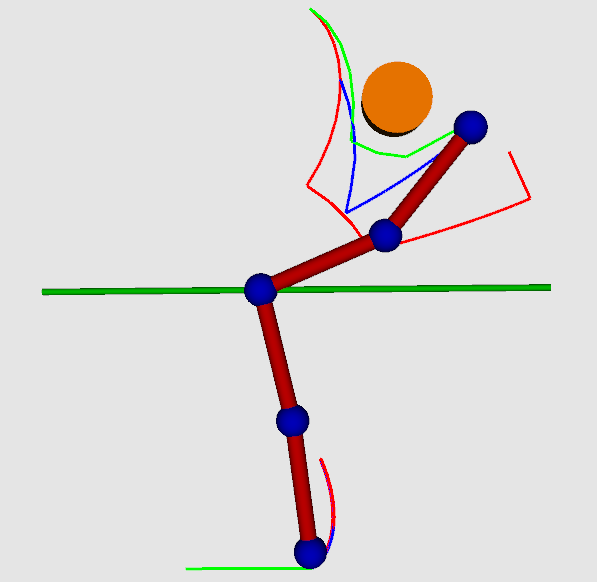
\includegraphics[width=6.5cm,height=5.5cm]{ur2_orth_constr_results.png}
    \caption*{Double-arm robot}
    \vspace{1ex}
  \end{minipage}%%
  \begin{minipage}[b]{0.5\linewidth}
    \centering
    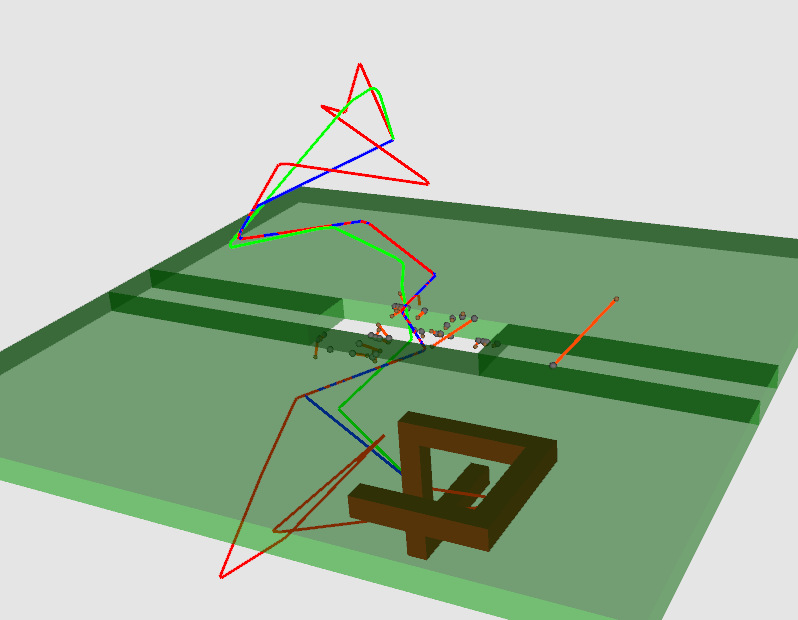
\includegraphics[width=6.5cm,height=5.5cm]{puzzle_orth_constr_results.png}
    \caption*{Freeflyer-puzzle robot}
    \vspace{1ex}
  \end{minipage} 
  \begin{minipage}[b]{0.5\linewidth}
    \centering
    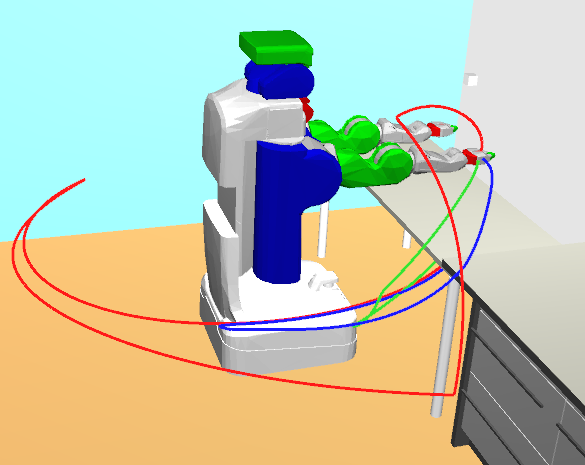
\includegraphics[width=6.5cm,height=5.5cm]{pr2-kitchen1_orth_constr_results.png}
    \caption*{PR2-in-kitchen-1}
    \vspace{1ex}
  \end{minipage}%% 
  \begin{minipage}[b]{0.5\linewidth}
    \centering
    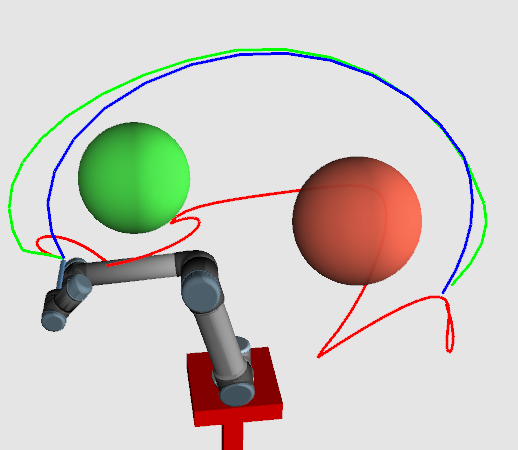
\includegraphics[width=6.5cm,height=5.5cm]{ur5-spheres_orth_constr_results.png}
    \caption*{UR5-with-spheres}
    \vspace{1ex}
  \end{minipage}
  \begin{minipage}[b]{0.5\linewidth}
    \centering
    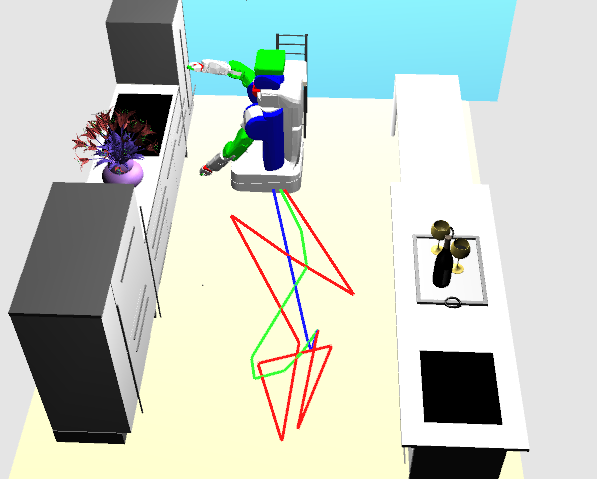
\includegraphics[width=6.5cm,height=5.5cm]{pr2_kitchen2_orth_constr_results.png}
    \caption*{PR2-in-kitchen-2}
  \end{minipage}%%
  \begin{minipage}[b]{0.5\linewidth}
    \centering
    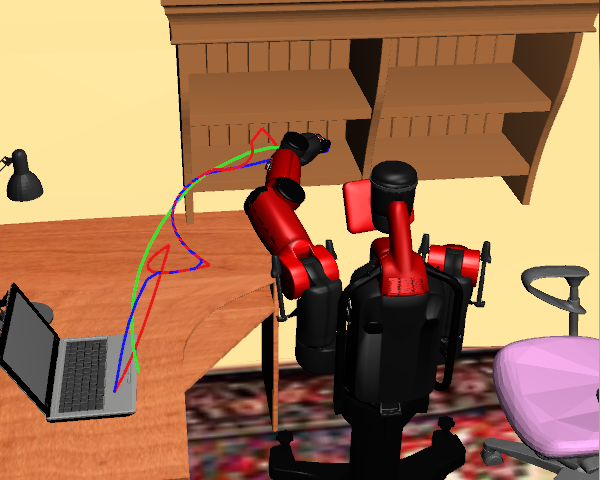
\includegraphics[width=6.5cm,height=5.5cm]{baxter_orth_constr_results.png}
    \caption*{Baxter-in-office}
  \end{minipage}
  \caption{Trajectories of end-effectors, mobile bases or centers allong the 
  different paths: the initial path is represented in red, the RS optimized path in 
  blue and the GB optimized path in green. The full robots 
  motions can also be visualized in the joined video. The trajectories comparison 
  highlights the optimization sucess of our method, which manages to deliver a 
  shorter or similar path compared to RS output}
  \label{fig:trajectories}
\end{figure}



\begin{table}
\centering
\scalebox{0.9}{
  \begin{tabular}{ccccc}
  \toprule
    \textbf{Problem} & Path obtained from & Computation time  & Path length & Base traveled distance\\
    \midrule
    \midrule
    & Initial &  & $21.9$  &\\
    \textbf{2D slidding-robot} & GB & $9.29\,\text{ms}$ & $17.0$  &\\
    \textbf{(Fig.~\ref{2D_long} right)} & PRS & $0.336\,\text{ms}$ & $21.7$  &\\
    & RS & $1.89\,\text{ms}$ & $6.05$  &\\
    \midrule
    & Initial &  & $ $  &\\
    \textbf{Freeflyer-} & GB & $\,\text{ms}$ & $ $  &\\
    \textbf{puzzle} & PRS & $\,\text{ms}$ & $ $  &\\
    & RS & $\,\text{ms}$ & $ $  &\\
    \midrule
    & Initial &  & $10.8$  &\\
    \textbf{Double-arm} & GB & $10.3\,\text{ms}$ & $4.79$  &\\
    \textbf{5-DOF} & PRS & $2.17\,\text{ms}$ & $8.08$  &\\
    & RS & $5.33\,\text{ms}$ & $6.24$  &\\
    \midrule
    & Initial &  & $12.6$  & $9.57$\,\text{m}\\
    \textbf{PR2-crossing-} & GB & $1.28\,\text{s}$ & $2.57$  & $0\,\text{m}$\\
    \textbf{arms} & PRS & $2.63\,\text{s}$ & $ 5.31$ & $0\,\text{m}$\\
    & RS & $1.92\,\text{s}$ & $3.59$ & $2.63\,\text{m}$\\
    \midrule
    & Initial &  & $15.3$ &\\
    \textbf{PR2-in-} & GB & $19.2\,\text{s}$ & $4.53$ &\\
    \textbf{kitchen-1} & PRS & $23.5\,\text{s}$ & $12.2$ &\\
    & RS & $9.88\,\text{s}$ & $5.75$ &\\
    \midrule
    & Initial &  & $ $ &\\
    \textbf{UR5-} & GB & $\,\text{s}$ & $ $ &\\
    \textbf{with-spheres} & PRS & $\,\text{s}$ & $ $ &\\
    & RS & $\,\text{s}$ & $ $ &\\
    \midrule
    & Initial &  & $ $ &\\
    \textbf{UR5-} & GB & $\,\text{s}$ & $ $ &\\
    \textbf{industrial-example} & PRS & $\,\text{s}$ & $  $ &\\
    & RS &  $\,\text{s}$ & $ $ &\\
    \midrule
    & Initial &  & $ $ &\\
    \textbf{Baxter-in-} & GB & $\,\text{s}$ & $ $ &\\
    \textbf{office} & PRS & $\,\text{s}$ & $ $ &\\
    & RS & $\,\text{s}$ & $ $ &\\
    \bottomrule
  \end{tabular}
  }%scalebox
\caption{Average results for 30 runs of several examples presented in the paper or 
the video. For each run, a solution path is planned by Visibility-PRM as initial 
guess for each optimizer.
For the PR2-crossing-arms example only, the right column represents the 
distance that is traveled by the robot mobile base during the different paths.
}
\label{tab:results}
\end{table}



\section{CONCLUSIONS}
We managed to settle a path optimization for decoupled-DOF robots such as mobile 
manipulators. Our algorithm uses standard numerical tools as collision checking 
and QP resolution, and correlates them in a 
simple but effective way, playing on the scalar iteration parameter. Therefore, 
our method only require few distances computation, so geometry pre-processing or 
offline optimization are not necessary to remain time competitive. We demonstrate 
that the optimizer is 
time-competitive comparing to random shortcut and proposes better quality paths 
for high-DOF robots, removing unnecessary DOF motions. Our optimizer also manages 
to reduce a local detour in a long path while random shortcut methods will mostly 
fail.

In a future work, we plan to study a combination of a random shortcut and the gradient-based optimizers since they seem to share a complementarity. .....

\bibliographystyle{tADR} % plain, alpha, abbr, unsrt
\bibliography{paper}

\end{document}
